\begin{figure}
    \centering
    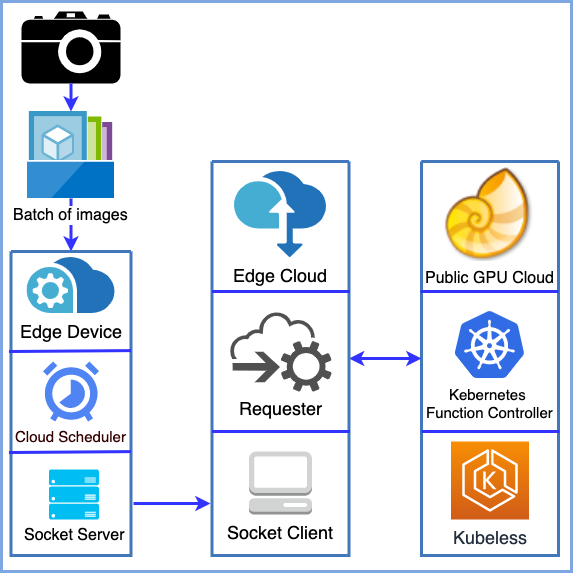
\includegraphics[scale=0.4]{STOIC}
    \caption{The STOIC Architecture \label{fig:STOIC}}
\end{figure}

To leverage hardware acceleration and distributed scheduling within a serverless architecture, we have developed STOIC, a framework for executing analytics applications in multi-tier IoT (sensing-edge-cloud) settings. STOIC streamlines the end-to-end process of packaging, transferring, scheduling, executing, and result retrieval for machine learning applications. Figure~\ref{fig:STOIC} shows three principal pillars of STOIC's architecture: Edge Controller, Edge Cloud, and Public Cloud.

\subsection{Edge Controller}
 We deploy a collection of edge devices, including multiple motion-detecting camera traps in open field and a local server as edge controller in the research facility at Sedgwick Natural Reserve~\cite{ref:sedgwick}. 
In this deployment, we install motion-triggered cameras (i.e. camera traps) at 
watering holes to capture images of wildlife in their natural habitat (as part of conservation science studies). The cameras are connected via a wireless radio to a computer located in an outbuilding at the reserve. We refer to this computer as the edge controller.  It is connected to a private campus cloud via a microwave link. When a camera trap detects motion, it takes photos and persists the images in flash storage. Periodically, the camera traps transfer saved photos to the edge controller. STOIC runs on the edge controller and its execution is triggered by the arrival of batches of images from camera traps located across the reserve. When a batch arrives, STOIC partitions the image processing application (for object/animal classification) into tasks that it assigns to 1+ cloud components.
 
 \subsection{Edge Cloud}
 
As an intermediate computational tier between the sensors and the public cloud, the edge cloud can be placed anywhere, preferably near the edge devices, to lower the response latency of analytics applications processing the images. Our edge cloud is currently deployed in our lab on campus which is connected to the edge controller via a fast network link.

Our edge cloud consists of a cluster of nine Intel NUCs~\cite{ref:nucs}.
Eucalyptus cloud system~\cite{ref:euca} manages the edge cloud and supports Linux virtual machine instances. Running on an instance, the STOIC socket client listens for the request from edge controller and then either executes the job locally on edge cloud or has STOIC requester interact with public cloud to complete the designated task.
 
 \subsection{Remote Public/Private Cloud}

To investigate the use of the serverless architecture with hardware accelerators, we employ a shared, multi-university, GPU cloud Nautilus~\cite{ref:nautilus} as our remote cloud system. Nautilus is an Internet-connected, HyperCluster research platform led by researchers at UC San Diego, National Science Foundation, the Department of Energy, and various participating universities globally.  Being designed for running data and computationally intensive applications, Nautilus uses Kubernetes~\cite{ref:k8s} as an interface to manage and scale containerized applications.  It uses Rook~\cite{ref:rook} to integrate Ceph~\cite{ref:ceph} data services. As of Nov. 2019, Nautilus consists of 141 computing nodes across the US and 422 GPUs are available in the cluster. All of these nodes are connected via a multi-campus network. In this study, we consider Nautilus as a public cloud that enables us to leverage hardware acceleration (GPUs) in the serverless architecture to serve edge devices. 
 
 \subsection{Implementation}
 
 Considering performance and interface, we
implement STOIC using Golang~\cite{ref:golang}. Golang provides high 
performance (vs scripting languages)and a user-friendly 
interface~\cite{ref:client-go} to Kubernetes.  STOIC currently supports machine learning applications developed using the TensorFlow  framework~\cite{ref:tensorflow}.
 
 \BlankLine
 \subsubsection{Serverless framework}
 For our serverless architecture, STOIC employs 
kubeless~\cite{ref:kubeless} and Docker~\cite{ref:docker} in the
 Nautilus Cloud. As a Kubernetes-native serverless framework, 
kubeless uses the Custom Resource Definition (CRD)\cite{ref:crd} to dynamically create functions as Kubernetes custom resources and launches runtimes on-demand. For specific machine learning tasks that STOIC executes, we use Docker to build customized runtime images that we upload to Docker 
Hub~\cite{ref:dockerhub} in advance. When the function controller 
at Nautilus Cloud receives a task request, it pulls the latest image 
from Docker Hub before launching the function. This deployment pipeline 
makes the runtime flexible and extensible for evolving applications. 
 
For the edge cloud, we execute tasks by directly invoking
the application function binaries. We make this design decision to simplify STOIC's control plane in  our prototype but we are investigating the use of
a consistent serverless architecture across edge and public/private 
cloud as part of future work.
 
 \BlankLine
 \subsubsection{STOIC Library Support}
 To leverage the computational power of the CPU systems available 
in the Edge and Public Cloud, we compile Tensorflow from source with AVX2, SSE4.2~\cite{ref:avx} and FMA~\cite{ref:fma} instruction set support. We then test the performance of customized Tensorflow package on three common machine learning training tasks: \textbf{(A)} \textit{Iris}~\cite{ref:iris} with 10-fold cross-validation; \textbf{(B)} \textit{MNIST}~\cite{ref:mnist} on 20 Epochs; \textbf{(C)} \textit{InceptionV3}~\cite{ref:v3} on 10 epochs with 1,000 images. 

We execute these applications 10 times on standard and customized Tensorflow packages. Table~\ref{tab:avx} shows the mean execution time of three benchmarks 
for each package. We calculate speed-up as $(T_s - T_c) / T_s$, where $T_s$ and $T_c$ represent the execution time by the standard and customized Tensorflow library respectively. We observe that, in all three benchmarks, the customized library achieves a speed-up that ranges from 17.4\% to 29.5\%. STOIC uses
the customized TensorFlow packages for cloud systems that implement these
instruction sets.  In our prototype, both the edge and public cloud have
these extensions.
 
 \BlankLine
 \subsubsection{GPU Accessibility}
 To enable GPU access by serverless functions, we build a container with NVIDIA Container Toolkit~\cite{ref:nvidia} support.  Such support includes the NVIDIA runtime library and utilities which link serverless functions to NVIDIA GPUs. We also install CUDA 10.0 and cuDNN 7.0 in the image.
 
\begin{table}
\centering
\captionsetup{justification=centering}
\caption{ \hspace{0pt} \\
\textsc{Performance Comparison on Three Benchmarks Between Standard and Custom Tensorflow Library Compiled with AVX2 / SSE / FMA CPU Instruction Set Support}}
\scriptsize

\begin{tabular}{|c|c|c|c|} 
\hline
 & \textbf{Mean Std. (sec)} & \textbf{Mean Custom. (sec)} & \textbf{Speed-up \%}\\
\hline
\textbf{Iris} & 53.17 & 41.86 &  21.3\\
\hline
\textbf{MNIST} & 268.81 & 189.80 & 29.4 \\
\hline
\textbf{InceptionV3} & 958.47 & 791.28 & 17.4 \\
\hline
\end{tabular}

\label{tab:avx}
\end{table}
 
 \BlankLine
 \subsubsection{STOIC Runtime}
 To schedule the machine learning tasks across hybrid cloud deployments, we define four runtime scenarios: \textbf{(A)} \textit{edge} - A VM instance on the edge cloud with AVX2 support; \textbf{(B)} \textit{cpu} - A Kubernetes pod on Nautilus containing a single CPU with AVX2 support; \textbf{(C)} \textit{gpu1} - A Kubernetes pod on Nautilus containing a single GPU; \textbf{(D)} \textit{gpu2} - A Kubernetes pod on Nautilus containing two GPUs. STOIC considers each of these deployment options as part of its scheduling decisions. Users can parameterize STOIC with their choice of deployment or allow STOIC to automatically schedule their applications.
 
 %For evaluation and canary deployment purpose, STOIC has implemented a feature flag of runtime that overrides the runtime selection made by scheduler when the user manually set the flag. This feature extensively helps evaluate the performance of STOIC, comparing with single-runtime schedulers.
 
 % STOIC executes tasks on the edge and cloud system for a warm up period (parameterizable but currently set to 1 hour) during which it observes deployment and execution times.
 
 \subsection{Execution Time Estimation}
 As depicted in Figure~\ref{fig:STOIC}, the STOIC socket server executes in the edge cloud and listens for requests from the edge controller (machine learning job requests). After a preset period (parameterizable but currently set to 1 hour), STOIC estimates total response time~($T_r$) of a requested batch, based on 4 different runtime scenarios. The total response time includes data transfer time~($T_t$), runtime deployment time~($T_d$) and corresponding processing time~($T_p$):
 
 \subsubsection{Transfer time~($T_t$)} measures the time spent in transmitting a compressed batch of images from the edge controller to edge cloud and public cloud. We calculate transfer time as ${T_t = F_b / B_c}$ where $F_b$ represents the file size of batch and $B_c$ represents the bandwidth at the moment provided by a bandwidth monitor at the edge controller. 
 
 \subsubsection{Runtime deployment time~($T_d$)} It measures the time Nautilus uses to deploy requested kubeless function. Since the scarcity of computation, it is common that \textit{gpu2} runtime takes longer to deploy than \textit{gpu1} and \textit{cpu} runtimes. We analyze the deployment log and calculate the average deployment time for each Nautilus runtime. In future work, we plan to develop a feedback control loop to dynamically update deployment time for each runtime. Note that, for \textit{edge} runtime, the transfer and runtime deployment time zero out since STOIC executes the task locally in the edge cloud.
 
 \subsubsection{Processing time~($T_p$)} is the execution time of a specific machine learning task. As a primary component for scheduling tasks across the hybrid cloud, we regress processing time based on prior experiment data by Bayesian Ridge Regression~\cite{ref:brr} due to its robustness to ill-posed problems compared to Ordinary Least Squares regression~\cite{ref:ols}. Thus, STOIC formulates the regression and uses it to predict the processing time based on the file size of the current batch. %Similarly to the runtime deployment time, we plan to construct a feedback control loop to dynamically update the coefficient and intercept of regression based on the incoming data of processing time as future work.
 
 \subsection{Workflow}
 The STOIC workflow is as follows: based on the three time components, STOIC predicts the total response times~($T_r$) of the four deployment options. The scheduler selects the runtime with the shortest estimated response time. Then the edge controller sends a request, including the payload of compressed image batch and runtime information, to edge cloud. Upon acceptance, the edge cloud executes the task locally if the choice is the \textit{edge} runtime. Such deployment is common when a batch of images is small. 

For large batch sizes, STOIC typically schedules one of the three public runtime options. For these three scenarios, the edge cloud first requests the deployment on the public cloud. It then sends the payload to public cloud storage. The public cloud then deploys and executes the kubeless function. As a design decision, instead of running a requester pod in the public cloud, we run an instance on the edge cloud. We do so because the edge cloud is more stable and fault resilient than Nautilus which experiences intermittent downtime.  
 
Once Nautilus successfully deploys the serverless function, it informs the edge cloud's requester to trigger the function via an HTTP request. When the task completes, the requester retrieves the results and runtime metrics, and transmits them back to the edge controller. Finally, the controller saves the results and metrics to persistent storage. 
 
 \subsection{Intelligent Probing}
 With a series of experiments, we have found that the processing times from the same image batch and kubeless function can vary significantly between the first run and successive runs. This is due to the differences between cold and warm starts~\cite{ref:coldstart}.  A cold start is when a machine learning task requires retrieval of stored model and dataset from cloud storage, which takes time. Once the function retrieves and caches this information, successive invocations of the function (using the same container) avoid this cost (i.e. experience a warm start). 

STOIC accounts for cold and warm starts in its scheduling estimate using intelligent probes. When STOIC schedules an incoming task in a different runtime than the previous one, it triggers the function with the least amount of input data to ensure the function caches the model and dataset in memory. Following this, STOIC triggers the actual tasks. To avoid redundant probing, STOIC starts the task directly when the designated runtime is the same as the previous batch.
